% ============================================================
%  DesignDen – Database Schema  (LaTeX)
%  Compile with:  pdflatex database_schema.tex
%  Requires packages: geometry, booktabs, longtable, xcolor,
%                     tikz, pgf, array, multirow, hyperref,
%                     fontawesome5 (optional), listings
% ============================================================
\documentclass[a4paper,11pt]{article}

% ── Packages ────────────────────────────────────────────────
\usepackage[a4paper, margin=2cm, top=2.5cm, bottom=2.5cm]{geometry}
\usepackage{booktabs}
\usepackage{longtable}
\usepackage[table]{xcolor}
\usepackage{array}
\usepackage{multirow}
\usepackage{hyperref}
\usepackage{tikz}
\usetikzlibrary{er, arrows, shapes, positioning, fit, calc}
\usepackage{listings}
\usepackage{parskip}
\usepackage{titlesec}
\usepackage{fancyhdr}
\usepackage{graphicx}
\usepackage{tabularx}
\usepackage{mdframed}
\usepackage{enumitem}

% ── Colours ─────────────────────────────────────────────────
\definecolor{primary}{HTML}{667eea}
\definecolor{secondary}{HTML}{764ba2}
\definecolor{success}{HTML}{4CAF50}
\definecolor{warning}{HTML}{FFC107}
\definecolor{danger}{HTML}{F44336}
\definecolor{info}{HTML}{2196F3}
\definecolor{darkbg}{HTML}{1a202c}
\definecolor{lightgray}{HTML}{f7f8fa}
\definecolor{tabhead}{HTML}{e8eaf6}
\definecolor{rowodd}{HTML}{f3f4ff}
\definecolor{roweven}{HTML}{ffffff}

% ── Hyperref setup ───────────────────────────────────────────
\hypersetup{
  colorlinks=true,
  linkcolor=primary,
  urlcolor=primary,
  pdftitle={DesignDen Database Schema},
  pdfauthor={DesignDen Team},
}

% ── Section formatting ───────────────────────────────────────
\titleformat{\section}{\large\bfseries\color{primary}}{}{0em}{}[\titlerule]
\titleformat{\subsection}{\normalsize\bfseries\color{secondary}}{}{0em}{}
\titleformat{\subsubsection}{\small\bfseries\color{darkbg}}{}{0em}{}

% ── Header / Footer ──────────────────────────────────────────
\pagestyle{fancy}
\fancyhf{}
\lhead{\textcolor{primary}{\textbf{DesignDen}} \textcolor{gray}{-- Database Schema}}
\rhead{\textcolor{gray}{\small March 2026}}
\cfoot{\textcolor{gray}{\thepage}}
\renewcommand{\headrulewidth}{0.4pt}

% ── Column types ─────────────────────────────────────────────
\newcolumntype{L}[1]{>{\raggedright\arraybackslash}p{#1}}
\newcolumntype{C}[1]{>{\centering\arraybackslash}p{#1}}

% ── Custom commands ──────────────────────────────────────────
\newcommand{\pk}{\textcolor{success}{\textbf{PK}}}
\newcommand{\fk}{\textcolor{warning}{\textbf{FK}}}
\newcommand{\uk}{\textcolor{info}{\textbf{UK}}}
\newcommand{\coll}[1]{\textcolor{primary}{\texttt{\textbf{#1}}}}
\newcommand{\dtype}[1]{\textcolor{secondary}{\texttt{#1}}}

% ── Listings (code) ───────────────────────────────────────────
\lstset{
  basicstyle=\ttfamily\footnotesize,
  backgroundcolor=\color{lightgray},
  frame=single,
  rulecolor=\color{primary!40},
  breaklines=true,
  keywordstyle=\color{primary}\bfseries,
  commentstyle=\color{gray}\itshape,
  stringstyle=\color{success},
}

% ─────────────────────────────────────────────────────────────
\begin{document}

% ── Title Page ───────────────────────────────────────────────
\begin{titlepage}
  \centering
  \vspace*{2cm}
  {\Huge\bfseries\textcolor{primary}{DesignDen}\par}
  \vspace{0.4cm}
  {\large\textcolor{secondary}{Custom Clothing E-Commerce Platform}\par}
  \vspace{1.5cm}
  \begin{mdframed}[linecolor=primary,linewidth=2pt,innertopmargin=16pt,innerbottommargin=16pt]
    \centering
    {\LARGE\bfseries Database Schema}\par
    \vspace{0.3cm}
    {\normalsize Entity Relationship Diagram}\par
    \vspace{0.3cm}
    {\small 15 MongoDB Collections $\cdot$ 5 User Roles $\cdot$ 16 Order Statuses}
  \end{mdframed}
  \vspace{2cm}
  \begin{tabular}{rl}
    \textbf{Database}   & MongoDB (Mongoose ODM)        \\[4pt]
    \textbf{Collections}& 15                            \\[4pt]
    \textbf{Version}    & 1.0.0                         \\[4pt]
    \textbf{Date}       & March 2026                    \\
  \end{tabular}
  \vfill
  {\small\textcolor{gray}{DesignDen Development Team}}
\end{titlepage}

\tableofcontents
\newpage

% ─────────────────────────────────────────────────────────────
\section{Overview}

DesignDen uses \textbf{MongoDB} with \textbf{Mongoose ODM} and consists of \textbf{15 collections}
modelling users, orders, products, designs, messaging, cart, wishlist, notifications,
reviews, feedback, designer portfolios, earnings, payout requests, production milestones,
and delivery partners.

\begin{table}[h!]
\centering
\rowcolors{2}{rowodd}{roweven}
\begin{tabular}{@{}L{3.5cm}L{5cm}L{6cm}@{}}
\toprule
\rowcolor{tabhead}
\textbf{Statistic} & \textbf{Value} & \textbf{Notes} \\
\midrule
Collections     & 15            & All schemas versioned \\
User Roles      & 5             & customer, designer, manager, admin, delivery \\
Order Statuses  & 16            & Full lifecycle \\
Prod Milestones & 8 stages      & 12\%--100\% progress \\
Indexes         & 10+           & Query-optimised \\
\bottomrule
\end{tabular}
\caption{High-Level Schema Statistics}
\end{table}

% ─────────────────────────────────────────────────────────────
\section{Entity Relationships}

\subsection{Relationship Summary}

\begin{mdframed}[linecolor=primary!50,backgroundcolor=primary!5]
\begin{itemize}[noitemsep]
  \item \textbf{USERS} $\longrightarrow$ ORDERS, DESIGNS, MESSAGES, NOTIFICATIONS, CARTS, WISHLISTS, REVIEWS, FEEDBACKS, DESIGNER\_PORTFOLIOS, DESIGNER\_EARNINGS, DESIGNER\_PAYOUT\_REQUESTS
  \item \textbf{ORDERS} $\longrightarrow$ DESIGNS, PRODUCTION\_MILESTONES, MESSAGES; $\longleftarrow$ DELIVERY\_PARTNERS
  \item \textbf{PRODUCTS} $\longrightarrow$ CART\_ITEMS, WISHLIST\_ITEMS, REVIEWS
  \item \textbf{CARTS} $\longrightarrow$ CART\_ITEMS
  \item \textbf{WISHLISTS} $\longrightarrow$ WISHLIST\_ITEMS
\end{itemize}
\end{mdframed}

\subsection{ER Diagram (TikZ)}

\begin{center}
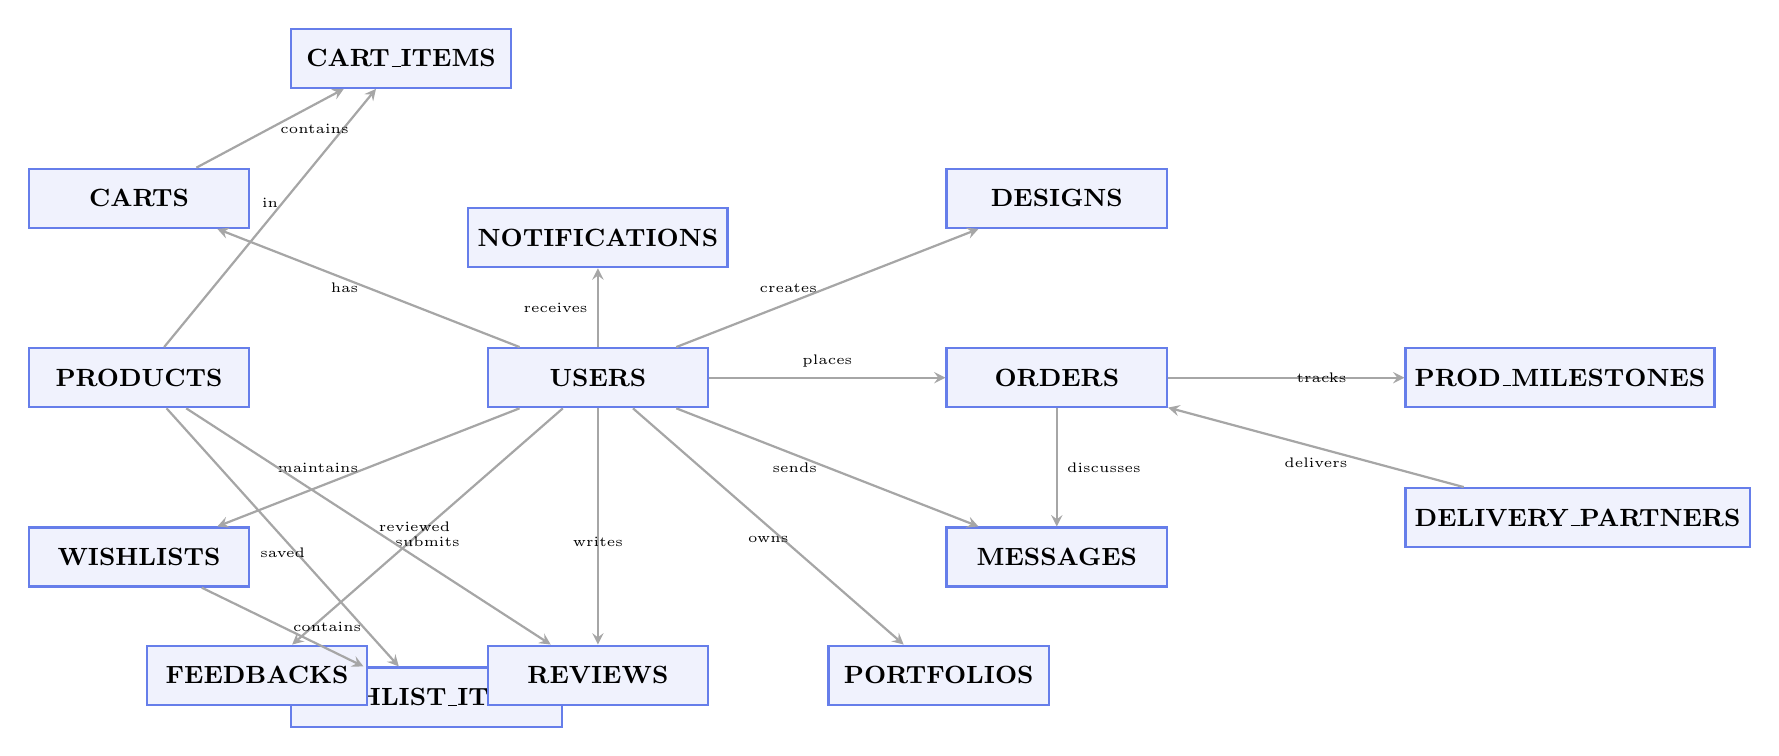
\begin{tikzpicture}[
  entity/.style={rectangle, draw=primary, fill=primary!10, thick,
                 minimum width=2.8cm, minimum height=0.75cm,
                 font=\small\bfseries},
  rel/.style={diamond, draw=secondary, fill=secondary!10, thick,
              aspect=2, font=\tiny},
  line/.style={->, >=stealth, thick, draw=gray!70},
  node distance=1.4cm and 2.2cm
]

  \node[entity] (users)      {USERS};
  \node[entity, right=3cm of users]  (orders)     {ORDERS};
  \node[entity, above=1.5cm of orders]  (designs)    {DESIGNS};
  \node[entity, below=1.5cm of orders]  (messages)   {MESSAGES};
  \node[entity, right=3cm of orders]  (milestones) {PROD\_MILESTONES};
  \node[entity, below right=1cm and 3cm of orders] (delivery)   {DELIVERY\_PARTNERS};
  \node[entity, left=3cm of users]  (products)   {PRODUCTS};
  \node[entity, above=1.5cm of products] (carts)      {CARTS};
  \node[entity, below=1.5cm of products] (wishlists)  {WISHLISTS};
  \node[entity, above right=1cm and 0.5cm of carts]  (cartitems) {CART\_ITEMS};
  \node[entity, below right=1cm and 0.5cm of wishlists] (wishitems) {WISHLIST\_ITEMS};
  \node[entity, above=1cm of users]   (notifs)     {NOTIFICATIONS};
  \node[entity, below=3cm of users]   (reviews)    {REVIEWS};
  \node[entity, left=1.5cm of reviews] (feedbacks)  {FEEDBACKS};
  \node[entity, right=1.5cm of reviews] (portfolios) {PORTFOLIOS};

  \draw[line] (users)    -- node[above,font=\tiny]{places}    (orders);
  \draw[line] (users)    -- node[left,font=\tiny]{creates}   (designs);
  \draw[line] (users)    -- node[left,font=\tiny]{sends}     (messages);
  \draw[line] (users)    -- node[left,font=\tiny]{receives}  (notifs);
  \draw[line] (users)    -- node[left,font=\tiny]{has}       (carts);
  \draw[line] (users)    -- node[left,font=\tiny]{maintains} (wishlists);
  \draw[line] (users)    -- node[below,font=\tiny]{writes}   (reviews);
  \draw[line] (users)    -- node[below,font=\tiny]{submits}  (feedbacks);
  \draw[line] (users)    -- node[below,font=\tiny]{owns}     (portfolios);
  \draw[line] (orders)   -- node[right,font=\tiny]{tracks}   (milestones);
  \draw[line] (orders)   -- node[right,font=\tiny]{discusses}(messages);
  \draw[line] (delivery) -- node[below,font=\tiny]{delivers} (orders);
  \draw[line] (products) -- node[above,font=\tiny]{in}       (cartitems);
  \draw[line] (products) -- node[below,font=\tiny]{saved}    (wishitems);
  \draw[line] (products) -- node[right,font=\tiny]{reviewed} (reviews);
  \draw[line] (carts)    -- node[right,font=\tiny]{contains} (cartitems);
  \draw[line] (wishlists)-- node[right,font=\tiny]{contains} (wishitems);

\end{tikzpicture}
\end{center}

% ─────────────────────────────────────────────────────────────
\section{Collection Schemas}

% ─── USERS ──────────────────────────────────────────────────
\subsection{\coll{users}}

\rowcolors{2}{rowodd}{roweven}
\begin{longtable}{@{}L{3.2cm}L{2.8cm}C{1.5cm}L{5.5cm}@{}}
\toprule
\rowcolor{tabhead}
\textbf{Field} & \textbf{Type} & \textbf{Key} & \textbf{Notes} \\
\midrule
\endfirsthead
\toprule
\rowcolor{tabhead}
\textbf{Field} & \textbf{Type} & \textbf{Key} & \textbf{Notes} \\
\midrule
\endhead
\bottomrule
\endlastfoot
\_id        & \dtype{ObjectId} & \pk  & Auto-generated primary key \\
email       & \dtype{String}   & \uk  & Unique index \\
password    & \dtype{String}   &      & bcrypt hashed \\
role        & \dtype{String}   &      & customer $|$ designer $|$ manager $|$ admin $|$ delivery \\
name        & \dtype{String}   &      & Display name \\
phone       & \dtype{String}   &      & Contact number \\
address     & \dtype{Object}   &      & Nested address object \\
isApproved  & \dtype{Boolean}  &      & Admin approval flag \\
isAvailable & \dtype{Boolean}  &      & Designer availability \\
createdAt   & \dtype{Date}     &      & Timestamp \\
\end{longtable}

% ─── ORDERS ─────────────────────────────────────────────────
\subsection{\coll{orders}}

\rowcolors{2}{rowodd}{roweven}
\begin{longtable}{@{}L{3.8cm}L{2.8cm}C{1.5cm}L{4.9cm}@{}}
\toprule
\rowcolor{tabhead}
\textbf{Field} & \textbf{Type} & \textbf{Key} & \textbf{Notes} \\
\midrule
\endfirsthead
\toprule
\rowcolor{tabhead}
\textbf{Field} & \textbf{Type} & \textbf{Key} & \textbf{Notes} \\
\midrule
\endhead
\bottomrule
\endlastfoot
\_id                & \dtype{ObjectId} & \pk & \\
customerId          & \dtype{ObjectId} & \fk & $\to$ users \\
designerId          & \dtype{ObjectId} & \fk & $\to$ users (designer) \\
deliveryPartnerId   & \dtype{ObjectId} & \fk & $\to$ delivery\_partners \\
orderType           & \dtype{String}   &     & shop $|$ custom \\
status              & \dtype{String}   &     & 16 states (see \S\ref{sec:statuses}) \\
items               & \dtype{Array}    &     & Order line items \\
totalAmount         & \dtype{Number}   &     & INR \\
deliveryOtp         & \dtype{String}   &     & 4-digit OTP \\
createdAt           & \dtype{Date}     &     & Timestamp \\
\end{longtable}

% ─── PRODUCTS ────────────────────────────────────────────────
\subsection{\coll{products}}

\rowcolors{2}{rowodd}{roweven}
\begin{tabular}{@{}L{3.2cm}L{2.8cm}C{1.5cm}L{5.5cm}@{}}
\toprule
\rowcolor{tabhead}
\textbf{Field} & \textbf{Type} & \textbf{Key} & \textbf{Notes} \\
\midrule
\_id      & \dtype{ObjectId} & \pk & \\
name      & \dtype{String}   &     & Product title \\
category  & \dtype{String}   &     & Clothing category \\
price     & \dtype{Number}   &     & INR \\
stock     & \dtype{Number}   &     & Inventory count \\
images    & \dtype{Array}    &     & Image URLs \\
isActive  & \dtype{Boolean}  &     & Listing status \\
\bottomrule
\end{tabular}

% ─── DESIGNS ─────────────────────────────────────────────────
\subsection{\coll{designs}}

\rowcolors{2}{rowodd}{roweven}
\begin{tabular}{@{}L{3.2cm}L{2.8cm}C{1.5cm}L{5.5cm}@{}}
\toprule
\rowcolor{tabhead}
\textbf{Field} & \textbf{Type} & \textbf{Key} & \textbf{Notes} \\
\midrule
\_id           & \dtype{ObjectId} & \pk & \\
orderId        & \dtype{ObjectId} & \fk & $\to$ orders \\
customerId     & \dtype{ObjectId} & \fk & $\to$ users \\
designerId     & \dtype{ObjectId} & \fk & $\to$ users \\
customization  & \dtype{Object}   &     & Fabric, colour, pattern, size \\
designFiles    & \dtype{Array}    &     & Uploaded design images \\
status         & \dtype{String}   &     & pending $|$ in\_progress $|$ completed $|$ approved $|$ rejected \\
createdAt      & \dtype{Date}     &     & \\
\bottomrule
\end{tabular}

% ─── MESSAGES ────────────────────────────────────────────────
\subsection{\coll{messages}}

\rowcolors{2}{rowodd}{roweven}
\begin{tabular}{@{}L{3.2cm}L{2.8cm}C{1.5cm}L{5.5cm}@{}}
\toprule
\rowcolor{tabhead}
\textbf{Field} & \textbf{Type} & \textbf{Key} & \textbf{Notes} \\
\midrule
\_id         & \dtype{ObjectId} & \pk & \\
orderId      & \dtype{ObjectId} & \fk & $\to$ orders \\
senderId     & \dtype{ObjectId} & \fk & $\to$ users \\
recipientId  & \dtype{ObjectId} & \fk & $\to$ users \\
content      & \dtype{String}   &     & Message text \\
type         & \dtype{String}   &     & text $|$ image $|$ file \\
isRead       & \dtype{Boolean}  &     & Read receipt flag \\
createdAt    & \dtype{Date}     &     & \\
\bottomrule
\end{tabular}

% ─── CART & CART ITEMS ───────────────────────────────────────
\subsection{\coll{carts} and \coll{cart\_items}}

\rowcolors{2}{rowodd}{roweven}
\begin{tabular}{@{}L{3.2cm}L{2.8cm}C{1.5cm}L{5.5cm}@{}}
\toprule
\rowcolor{tabhead}
\multicolumn{4}{l}{\textbf{carts}} \\
\midrule
\_id       & \dtype{ObjectId} & \pk & \\
userId     & \dtype{ObjectId} & \fk & $\to$ users \\
createdAt  & \dtype{Date}     &     & \\
\midrule
\rowcolor{tabhead}
\multicolumn{4}{l}{\textbf{cart\_items}} \\
\midrule
\_id        & \dtype{ObjectId} & \pk & \\
cartId      & \dtype{ObjectId} & \fk & $\to$ carts \\
productId   & \dtype{ObjectId} & \fk & $\to$ products \\
quantity    & \dtype{Number}   &     & \\
price       & \dtype{Number}   &     & Snapshot at add time \\
\bottomrule
\end{tabular}

% ─── REMAINING COLLECTIONS ───────────────────────────────────
\subsection{Other Collections}

\rowcolors{2}{rowodd}{roweven}
\begin{longtable}{@{}L{4.5cm}L{3.5cm}L{5cm}@{}}
\toprule
\rowcolor{tabhead}
\textbf{Collection} & \textbf{Key Fields} & \textbf{Purpose} \\
\midrule
\endfirsthead
\toprule
\rowcolor{tabhead}
\textbf{Collection} & \textbf{Key Fields} & \textbf{Purpose} \\
\midrule
\endhead
\bottomrule
\endlastfoot
\coll{wishlists}               & userId (\fk)              & Saved items per user \\
\coll{wishlist\_items}         & wishlistId, productId     & Individual saved products \\
\coll{notifications}           & userId (\fk), isRead      & User alert feed \\
\coll{reviews}                 & productId, userId, rating & Product reviews (1--5 stars) \\
\coll{feedbacks}               & userId, category, status  & Customer feedback \\
\coll{designer\_portfolios}    & designerId, images        & Designer showcase items \\
\coll{designer\_earnings}      & designerId, orderId, amount, commission & 80\% commission tracking \\
\coll{designer\_payout\_requests} & designerId, amount, status & Payout request management \\
\coll{production\_milestones}  & orderId, milestone, status & 8-stage progress tracking \\
\coll{delivery\_partners}      & name, phone, vehicleNumber & Delivery staff registry \\
\end{longtable}

% ─────────────────────────────────────────────────────────────
\section{Order Status States}
\label{sec:statuses}

The \coll{orders.status} field cycles through 16 states:

\begin{center}
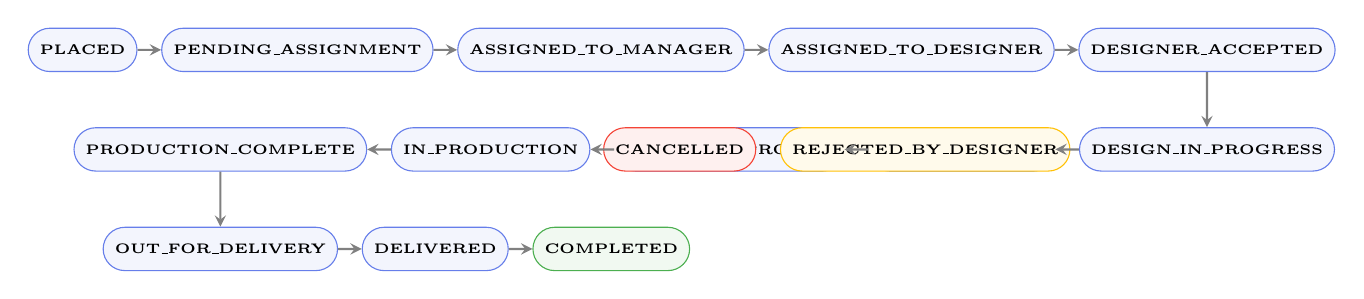
\begin{tikzpicture}[
  state/.style={rounded rectangle, draw=primary, fill=primary!8,
                font=\tiny\bfseries, minimum height=0.55cm,
                inner sep=4pt},
  arr/.style={->, >=stealth, draw=gray, thick},
  node distance=0.5cm and 0.3cm
]
  \node[state] (s1)  {PLACED};
  \node[state, right=of s1]  (s2)  {PENDING\_ASSIGNMENT};
  \node[state, right=of s2]  (s3)  {ASSIGNED\_TO\_MANAGER};
  \node[state, right=of s3]  (s4)  {ASSIGNED\_TO\_DESIGNER};
  \node[state, right=of s4]  (s5)  {DESIGNER\_ACCEPTED};
  \node[state, below=0.7cm of s5] (s6)  {DESIGN\_IN\_PROGRESS};
  \node[state, left=of s6]   (s7)  {DESIGN\_READY};
  \node[state, left=of s7]   (s8)  {DESIGN\_APPROVED};
  \node[state, left=of s8]   (s9)  {IN\_PRODUCTION};
  \node[state, left=of s9]   (s10) {PRODUCTION\_COMPLETE};
  \node[state, below=0.7cm of s10](s11) {OUT\_FOR\_DELIVERY};
  \node[state, right=of s11] (s12) {DELIVERED};
  \node[state, right=of s12, draw=success, fill=success!8] (s13) {COMPLETED};
  \node[state, below=0.7cm of s3,xshift=1cm, draw=danger, fill=danger!8]  (s14) {CANCELLED};
  \node[state, right=of s14, draw=warning, fill=warning!8] (s15) {REJECTED\_BY\_DESIGNER};
  \draw[arr] (s1)--(s2); \draw[arr] (s2)--(s3); \draw[arr] (s3)--(s4);
  \draw[arr] (s4)--(s5); \draw[arr] (s5)--(s6); \draw[arr] (s6)--(s7);
  \draw[arr] (s7)--(s8); \draw[arr] (s8)--(s9); \draw[arr] (s9)--(s10);
  \draw[arr] (s10)--(s11); \draw[arr] (s11)--(s12); \draw[arr] (s12)--(s13);
\end{tikzpicture}
\end{center}

% ─────────────────────────────────────────────────────────────
\section{Production Milestones}

\rowcolors{2}{rowodd}{roweven}
\begin{tabular}{@{}C{1cm}L{5cm}C{2.5cm}C{4cm}@{}}
\toprule
\rowcolor{tabhead}
\textbf{\#} & \textbf{Milestone Name} & \textbf{Progress \%} & \textbf{Status Values} \\
\midrule
1 & Material Procurement   & 12\%  & pending $|$ in\_progress $|$ completed \\
2 & Pattern Making         & 25\%  & pending $|$ in\_progress $|$ completed \\
3 & Cutting                & 37\%  & pending $|$ in\_progress $|$ completed \\
4 & Stitching              & 50\%  & pending $|$ in\_progress $|$ completed \\
5 & Assembly               & 62\%  & pending $|$ in\_progress $|$ completed \\
6 & Quality Check          & 75\%  & pending $|$ in\_progress $|$ completed \\
7 & Finishing              & 87\%  & pending $|$ in\_progress $|$ completed \\
8 & Final QC \& Packaging  & 100\% & pending $|$ in\_progress $|$ completed \\
\bottomrule
\end{tabular}

% ─────────────────────────────────────────────────────────────
\section{Collections Summary}

\rowcolors{2}{rowodd}{roweven}
\begin{longtable}{@{}L{4.8cm}L{4.5cm}L{4.7cm}@{}}
\toprule
\rowcolor{tabhead}
\textbf{Collection} & \textbf{Purpose} & \textbf{Key Relationships} \\
\midrule
\endfirsthead
\toprule
\rowcolor{tabhead}
\textbf{Collection} & \textbf{Purpose} & \textbf{Key Relationships} \\
\midrule
\endhead
\bottomrule
\endlastfoot
\coll{users}                      & User accounts (5 roles)      & Core entity \\
\coll{orders}                     & Order tracking (16 statuses) & users, designers, delivery \\
\coll{products}                   & Shop inventory               & cart/wishlist \\
\coll{designs}                    & Custom design data           & orders + designers \\
\coll{messages}                   & Chat system                  & users + orders \\
\coll{carts}                      & Shopping carts               & users + products \\
\coll{wishlists}                  & Saved items                  & users + products \\
\coll{notifications}              & User alerts                  & users \\
\coll{reviews}                    & Product reviews              & users + products \\
\coll{feedbacks}                  & Customer feedback            & users \\
\coll{designer\_portfolios}       & Designer showcase            & designers \\
\coll{designer\_earnings}         & Commission tracking          & designers + orders \\
\coll{designer\_payout\_requests} & Payout management            & designers \\
\coll{production\_milestones}     & Progress tracking            & orders \\
\coll{delivery\_partners}         & Delivery system              & orders \\
\end{longtable}

% ─────────────────────────────────────────────────────────────
\section{Indexes}

\begin{mdframed}[linecolor=primary!40, backgroundcolor=primary!4]
\begin{tabular}{@{}L{5cm}L{4cm}L{4cm}@{}}
\toprule
\rowcolor{tabhead}
\textbf{Index} & \textbf{Type} & \textbf{Rationale} \\
\midrule
\texttt{users.email}                        & Unique        & Login lookup \\
\texttt{orders.customerId}                  & Standard      & Customer orders \\
\texttt{orders.designerId}                  & Standard      & Designer orders \\
\texttt{orders.status}                      & Standard      & Filter by state \\
\texttt{designs.orderId}                    & Standard      & Design by order \\
\texttt{messages.orderId}                   & Standard      & Chat per order \\
\texttt{cart\_items.cartId}                 & Standard      & Cart load \\
\texttt{reviews.productId}                  & Standard      & Product reviews \\
\texttt{designer\_earnings.designerId}      & Standard      & Earnings query \\
\texttt{production\_milestones.orderId}     & Standard      & Progress lookup \\
\bottomrule
\end{tabular}
\end{mdframed}

\vfill
\begin{center}
  \small\textcolor{gray}{DesignDen $\cdot$ Database Schema $\cdot$ v1.0 $\cdot$ March 2026}
\end{center}

\end{document}
